\documentclass{article}
\usepackage[a4paper, total={6in, 27cm}]{geometry}
\usepackage{amsmath}
\usepackage{graphicx}

\begin{document}

\title{MATH 340}
\author{Quiz 1}
\date{\today}
\maketitle

\begin{enumerate}
	\item (5 points) True of False
		\begin{enumerate}
			\item (T)  (F)  The constant function $y'(x)=\pi$ is a
				solution of the ODE $y'(x)=x\sin^2(y)$.
			\item (T)  (F)  For the initial value problem
				$\begin{cases}
					x'(t)=2x+e^t\\
					x(0)=0
				\end{cases}$, the solution is $x(t)=e^{2t}-e^t$.
			\item (T)  (F)  The ODE $x'(t)+\sin(x(t))=0$ is linear.
			\item (T)  (F)  The ODE $x'(t)+\sin^2(x(t))=0$ is of order 2.
			\item (T)  (F)  The ODE $x'(t)+2tx(t)=0$ is linear.
		\end{enumerate}
	\item (5 points) The direction field of an ODE is shown below.
		\begin{center}
		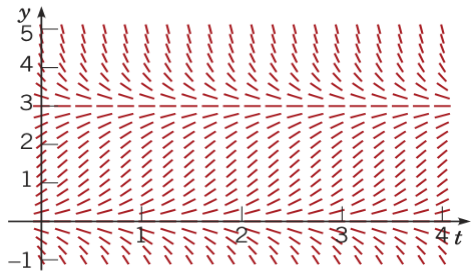
\includegraphics[width=0.5\textwidth]{quiz1DirField.png}
		\end{center}
		\begin{enumerate}
			\item Circle the differential equation that corresponds
				to the direction field. Briefly explain why.
			\[
				y'=y(y-3);\quad y'=y(3-y);\quad y'=y-3;\quad y'=y.
			\]
			\vspace{5cm}
			\item Based on the diagram identify two equilibrium
				points of the ODE (i.e. where the function
				stays constant).
		\end{enumerate}
\end{enumerate}

\end{document}
